\documentclass[../../../patent_v1.tex]{subfiles}

\begin{document}

\begin{figure*}
    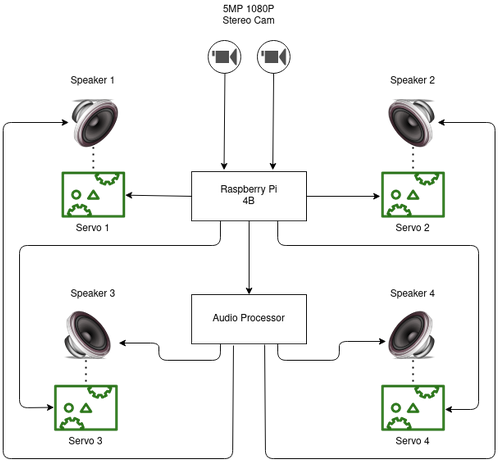
\includegraphics[width=\textwidth]{block_diagram.png}
    \caption{Block diagram}
\end{figure*}

\FloatBarrier

The dynamic audio system can be simplified as five measure blocks, each serving its 
own application in order to provide a dynamic surround pocket over the listener's head,

\section{Depth estimation unit}

\subfile{../depth_estimation_unit/depth_estimation_unit.tex}

\section{Micro-processor}

\subfile{../micro_processor/micro_processor.tex}

\section{Mechanical Unit}

\subfile{../mechanical_unit/mechanical_unit.tex}

\section{Audio Processing Unit}

\subfile{../audio_processing_unit/audio_processing_unit.tex}

\section{Speakers}

Speakers serve the four channeled dynamically adjusted surround sound to the listener. 
Usually, they are mounted on four corners of the room, either at the listener's ear 
levels or near the ceiling.

\end{document}